\section{Fases da missão de \gls{rvdb}}

A missão considerada neste trabalho segue a sequência típica de operações de \gls{rvdb} entre uma espaçonave perseguidora e uma espaçonave alvo em órbita circular, conforme descrito por \cite{fehse2003}. 
De forma geral, como apresentado na Figura~\ref{fig_etapas_rvdb}, a missão é composta pelas seguintes etapas:

\begin{figure}[H]
\centering
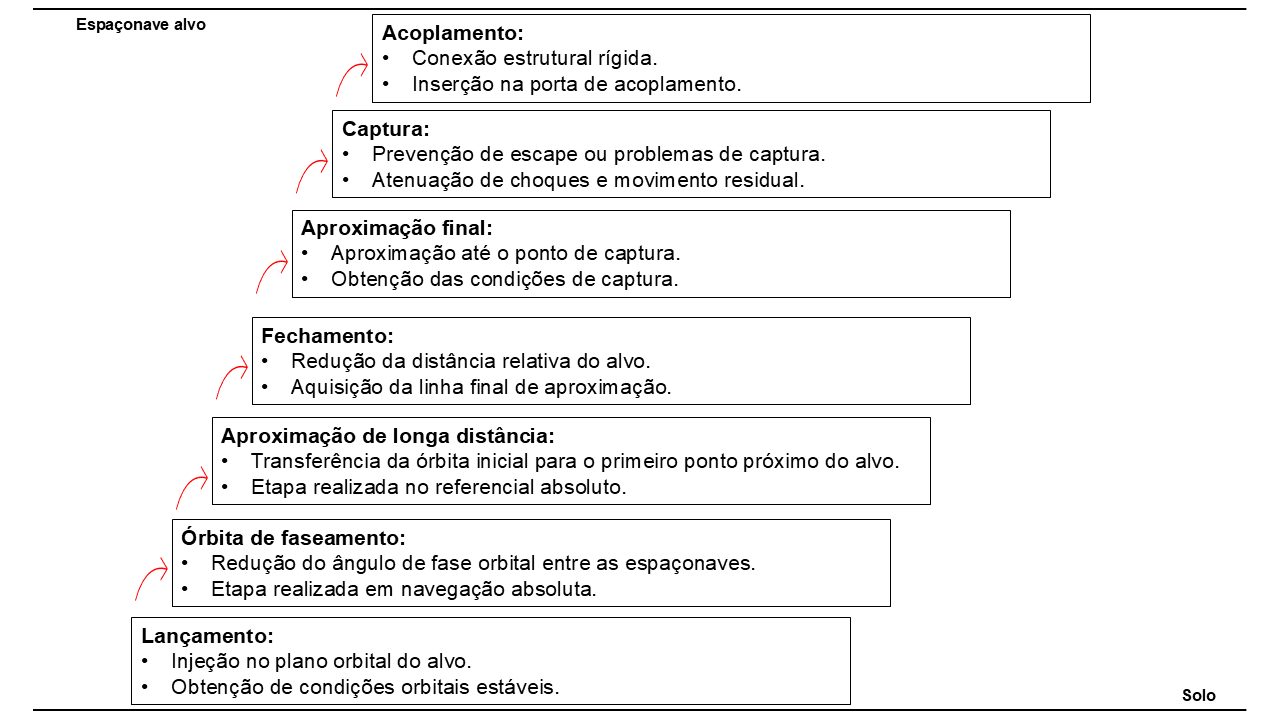
\includegraphics[width=1\linewidth]{4 Formulacao matematica/Imagens/Lançamento quadro explicativo.png}
\caption{Fases de uma missão de \gls{rvdb}, adaptado de \cite{fehse2003}.}
\label{fig_etapas_rvdb}
\end{figure}


\begin{itemize}
  \item lançamento e injeção do perseguidor em sua órbita inicial;
  \item redução da diferença do ângulo de fase entre as espaçonaves;
  \item aproximação de longa distância, realizada por meio de manobras de transferência orbital;
  \item início do movimento relativo entre as espaçonaves no referencial \gls{lvlh} centrado no alvo;
  \item execução das aproximações de curta distância e final;
  \item controle da atitude e da posição relativa do perseguidor, garantindo o alinhamento com a espaçonave alvo durante as etapas finais da aproximação.
\end{itemize}

A Figura~\ref{fig_fases_trabalho} apresenta a sequência da missão de \gls{rvdb} deste trabalho e que definem o fluxo operacional considerado na simulação.

\begin{figure}[H]
\centering
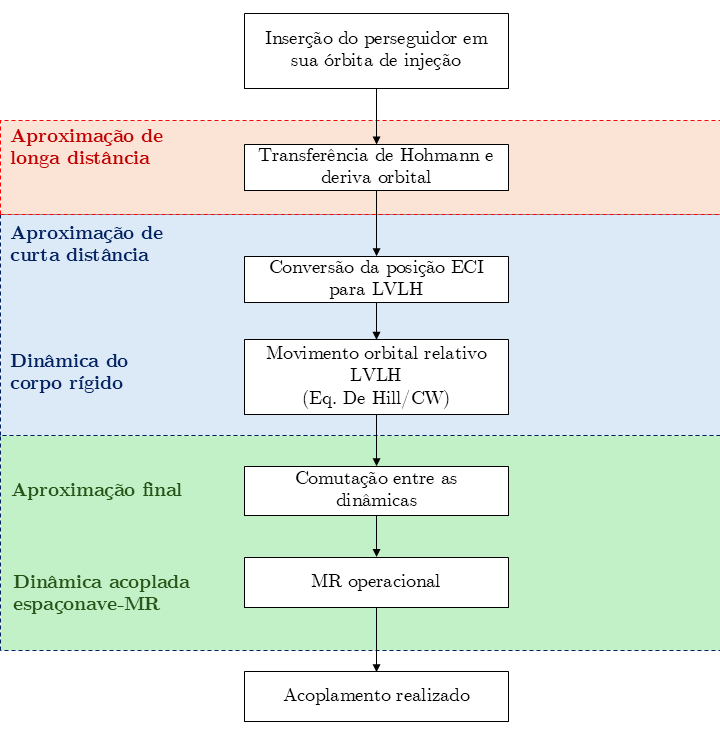
\includegraphics[width=1\linewidth]{3 Procedimento simulacao/Imagens diagrama/1 Geral.png}
\caption{Sequência das fases da missão de \gls{rvdb} deste trabalho.}
\label{fig_fases_trabalho}
\end{figure}



\section{Premissas adotadas para a simulação}

Nesta pesquisa, assume-se que o lançador realiza a injeção do perseguidor em uma órbita circular e coplanar à órbita do alvo, que simplifica a modelagem da dinâmica orbital.

A condição de coplanaridade está diretamente associada ao planejamento da janela de lançamento, que deve permitir a inserção do perseguidor em um plano orbital similar com o do alvo. 
Quando essa condição é satisfeita, a necessidade de manobras posteriores de correção do plano orbital é reduzida, permitindo concentrar a análise nas etapas de aproximação e movimento relativo entre as espaçonaves.